\documentclass[slidestop,compress,mathserif]{beamer}

%%% THEME

\usetheme{Antibes}
%\usetheme{Malmoe}
%\usetheme{Singapore}
%\usetheme{PaloAlto}
%\usetheme{AnnArbor}
%\usetheme{CambridgeUS}
%\usetheme{JuanLesPins}

%%% FOOTER

%\useoutertheme{infolines}

%%% COLOR

%\usecolortheme[RGB={170,255,64}]{structure}		% verde {170,255,0}
%\usecolortheme[RGB={255,108,0}]{structure}		% arancione
%\usecolortheme[RGB={0,102,255}]{structure}		% blu/azzurro
\usecolortheme[RGB={187,206,215}]{structure}		% blu insaturo
%\usecolortheme[RGB={192,192,192}]{structure}		% grigio

%%% PAGE NUMBERS

\setbeamertemplate{footline}[page number]
\setbeamertemplate{navigation symbols}


%%% PACKAGES 

\usepackage[italian]{babel}
\usepackage[latin1]{inputenc}
\usepackage{times}
\usepackage[T1]{fontenc}
\usepackage{verbatim}

%%% DOCUMENT META-DATA

\title{Traffic Simulator}
\author{Michael Gattavecchia \and Marco Santarelli \and Andrea Zagnoli}
\date{\today}
\institute{{\rm ALMA MATER STUDIORUM\\
		II Facolt\`a di Ingegneria - Sede di Cesena\\
		Tecnologie e Sistemi per la Sicurezza}}

%%% TABLE OF CONTENTS

%\AtBeginSubsection[]
%{
%\begin{frame}<beamer>{Sommario}
%\tableofcontents[currentsubsection]
%\end{frame}
%}

%%% DOCUMENT

\begin{document}

\frame{\titlepage}
\setcounter{tocdepth}{1}
\tableofcontents
\section{Introduzione}

\begin{frame}{Traffic Simulator}
\vfill
Realizzazione di un simulatore software di sistemi soggetti a traffico, in particolare di sistemi a singolo servitore e caratterizzati da una statistica del tempo di arrivo di tipo \emph{Poissoniano}
\vfill
Simulazione e presentazione dei relativi risultati di differenti aspetti concernenti tali sistemi (con la possibilit\`a di variarne i parametri al contorno)
 \begin{itemize}
 	\footnotesize
	\item generatori di numeri casuali
	\item simulatori $M/G/1$
	\item simulatori $M/G/1//Prio$
	\item simulatori $M/G/1//SJN$
 \end{itemize}
 \vfill
\end{frame}

\begin{frame}{Caratteristiche Simulator}
\vfill
In ambito generale \`e possibile classificare i simulatori secondo determinate propriet\`a; per quanto riguarda il \texttt{Simulator} di seguito implementato, esso \`e
 \begin{itemize}
 	\footnotesize
	\item[\textbullet] {\tt dinamico} a {\tt tempo asincrono}, il sistema evolve nel tempo, ma scorre in maniera irregolare
	\item[\textbullet] {\tt event-driven}, basato sul concetto di evento che determina i cambiamenti di stato del sistema, influisce sugli eventi futuri e sullo scorrere del tempo
	\item[\textbullet] {\tt statistico}, le grandezze in ingresso al simulatore sono di tipo aleatorio e quindi affette da incertezza statistica
	\item[\textbullet] {\tt continuo}, dato che le variabili di interesse che descrivono il sistema sono di tipo continue
 \end{itemize}
 \vfill
\end{frame}


\subsection{Gruppo di lavoro}

\begin{frame}{Gruppo di lavoro}
	\begin{block}{Componenti del gruppo}
	\begin{itemize}
		\item Michael Gattavecchia (\emph{n\slash m 0000362269})
		\item Marco Santarelli (\emph{n\slash m 0000346651})
		\item Andrea Zagnoli (\emph{n\slash m 0000367565})
	\end{itemize}
	\end{block}
\end{frame}

\section{Generazione di numeri casuali}
\begin{frame}{Generazione di numeri casuali}
\vfill
Alla base di una qualsivolglia simulazione risiede la centralit\`a del ruolo rivestito dalla riproduzione dell'aleatoriet\`a riscontrabile all'interno dei sistemi reali.
\vfill
Perci\'o risulta fondamentale valutare e conoscere le entit\`a alle quali si fa riferimento per la generazione di numeri casuali, il cui comportamento incider\`a in maniera rilevante sulla qualit\`a delle simulazioni.
\vfill
\end{frame}

\subsection{Generatori lineari congruenziali}

\begin{frame}{Generatori LC}
\vfill
$$
Z_{i}=(a \cdot Z_{i-1}+c)\mod m
$$
\vfill
Particolarmente apprezzati per la loro leggerezza, dovuta alla semplicit\`a dei calcoli necessari per la generazione. 

Esiste correlazione tra valori generati successivamente, che determina l'impossibilit\`a di utilizzo di questo tipo di generatori in ambienti in cui tale correlazione tappresenti un fattore di rischio (e.g. crittografia).
\vfill
\end{frame}

\subsection{Classe {\tt util.Random}}

\begin{frame}{\tt java.util.Random}
Rappresenta lo standard per la generazione di valori pseudo-random all'interno dell'invironment Java.
\begin{table}[!h]
	\begin{center}
	\begin{tabular}{c|c}
	parametro & valore\\
	\hline
	$m$ & $2^{48}$  \\
	$a$ & $25214903917$  \\
	$c$ & $11$  \\
	\end{tabular}
	\end{center}
	\caption{Parametri del LCG implementato in {\tt java.util.Random}}
	\label{tab:rndjava}
\end{table}
Presenta un periodo pari a $2^{48}$ ed utilizza un seme a $48$ bit per l'inizializzazione.
\end{frame}

\subsection{Generatore {\it ran0}}
\begin{frame}{Generatore ran0}
Generatore LC realizzato ex-novo.
\begin{table}[!h]
	\begin{center}
	\begin{tabular}{c|c}
	parametro & valore\\
	\hline
	$m$ & $2147483647$  \\
	$a$ & $16807$  \\
	$c$ & $0$  \\
	\end{tabular}
	\end{center}
	\caption{Parametri del LCG implementato ex-novo ({\tt RandomProvider})}
	\label{tab:rndcustom}
\end{table}
Il valore di $c=0$ ne fa un generatore ``moltiplicativo'', di tipo {\em Park-Miller}
\end{frame}

\subsection{Generatore {\tt MersenneTwister}}

\begin{frame}{{\tt MersenneTwister} / {\tt SecureRandom}}
\begin{block}{MersenneTwister}
Generatore implementato dal team Apache\footnote{http://www.apache.org}, implementa l'algoritmo  Matsumoto-Nishimura (1996-97). 
Basato sulla ricorsione lineare:
$x_{k+n}:=x_{k+m} \oplus (x_{k}^{u}|x_{k+1}^{l})A, (k=0,1,...)$
Caratterizzato da un periodo parcolarmente lungo (pari a $2^{19937}-1$), da una equidistribuzione a 623 dimensioni e da una accuratezza massima pari a 32 bit.
\end{block}
\begin{block}{SecureRandom}
Presente all'interno del package {\tt java.security} permette la generazione robusta dal punto di vista crittografico di numeri pseudo-casuali.
\end{block}
\end{frame}

\section{Analisi del generatore}
\subsection{Scatter Plot}
\begin{frame}{Valutazione della distribuzione [0,1]}
\vfill
Metodo per la valutazione visuale della distribuzione dei valori generati.

Coppie di valori vengono considerate come coordinate $x$ e $y$ e poste su di un piano cartesiano, in cui l'uniformit\`a di distribuzione dei valori nello spazio sar\`a indicatore della qualit\`a del generatore.
\vfill
\end{frame}

\begin{frame}{Scatter plot}
\begin{figure}[!h]{
	\begin{center}
	   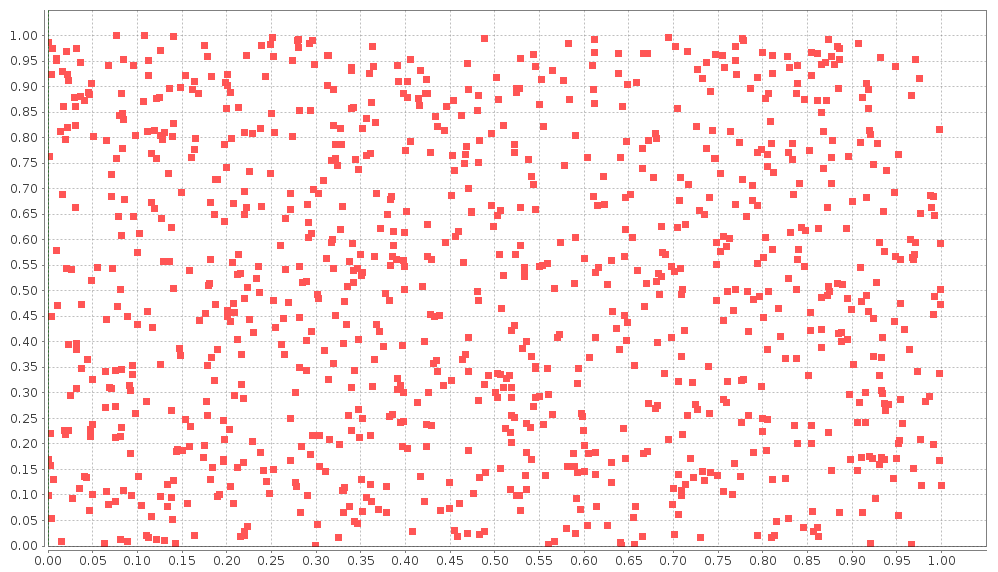
\includegraphics[width=0.9\textwidth]{figures/random.png}
	\end{center}}
	\caption{Distribuzione dei valori generati da {\tt util.Random}}
	\label{fig:random}
\end{figure}
\end{frame}

\subsection{Stima del valore medio}
\begin{frame}{Stima del valore medio}
\vfill
Al fine di valutare il valore medio delle serie di valori prodotti sono state effettuate alcune serie di generazioni di campioni di dimensione crescente.

All'aumentare della numerosit\`a dei campioni si nota la convergenza della media al valore teorico $0.5$.

Si notano oscillazioni rilevanti esclusivamente in concomitanza a campioni di dimensioni ridotte.
\vfill
\end{frame}

\begin{frame}{Media dei campioni}
\begin{figure}[!h]{
	\begin{center}
	   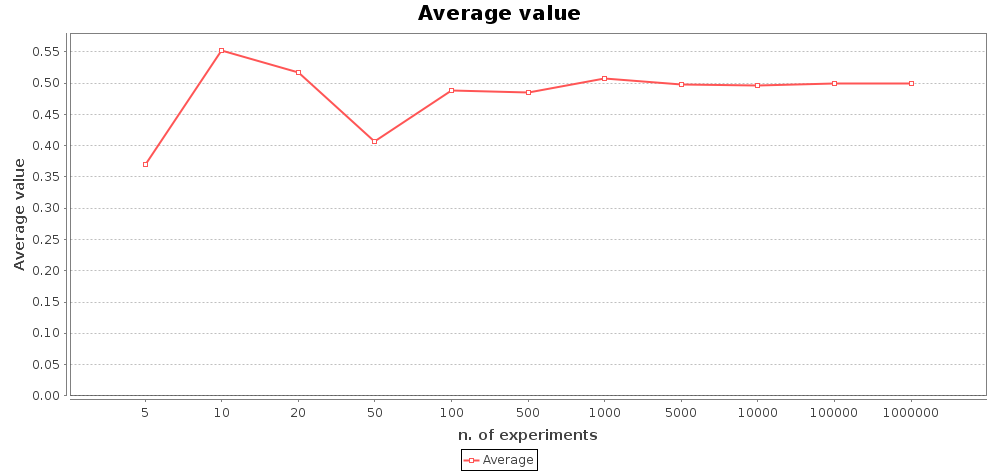
\includegraphics[width=0.95	\textwidth]{figures/average.png}
	\end{center}}
	\caption{Media dei campioni in funzione della numerosit\`a}
	\label{fig:avg}
\end{figure}
\end{frame}

\subsection{Intervallo di confidenza}
\begin{frame}{Intervallo di confidenza (1/2)}
L'intervallo di confidenza \`e stato valutato in funzione del livello di confidenza richiesto...
\begin{figure}[!h]{
	\begin{center}
	   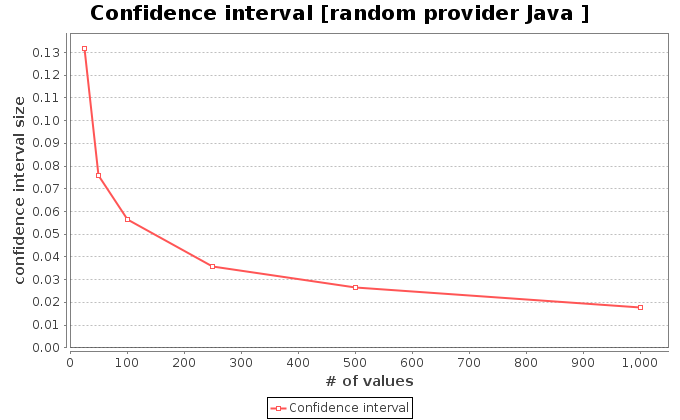
\includegraphics[width=0.8\textwidth]{figures/IDC_1.png}
	\end{center}}
	\caption{Intervallo di confidenza in funzione del numero di campioni}
	\label{fig:idce1}
\end{figure}
\end{frame}

\begin{frame}{Intervallo di confidenza (2/2)}
...ed al variare della dimensione dei campioni
\begin{figure}[!h]{
	\begin{center}
	   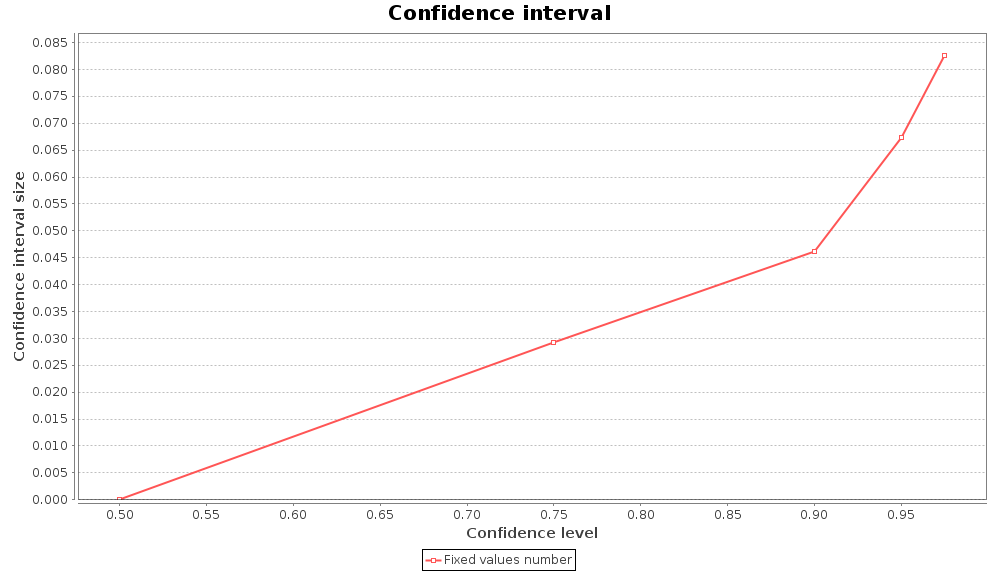
\includegraphics[width=0.8\textwidth]{figures/IDC_2.png}
	\end{center}}
	\caption{Intervallo di confidenza in funzione del livello di confidenza}
	\label{fig:idc2}
\end{figure}
\end{frame}

\begin{frame}{Analisi tecnica}
\vfill
Le simulazioni relative all'intervallo di confidenza sono state realizzate attraverso i metodi:
\begin{itemize}
\footnotesize
\item {\tt testConfidenceIntervalWithVariableConfidence(...)} 
\item {\tt testConfidenceIntervalWithVariableRuns(...)}
\end{itemize} 
\normalsize
della classe {\tt SimulationRunners}, che contiene i metodi utilizzati per svolgere le varie tipologie di simulazioni disponibili.
\vfill
\end{frame}

\section{Modelli di traffico}
\begin{frame}{Generazione di traffico}
\vfill
Generazione di eventi secondo differenti distribuzioni
\begin{itemize}
		\item Deterministico
		\item Esponenziale
		\item SPP
		\item Pareto
\end{itemize}
Parametri di traffico scelti in modo da ottenere per ogni distribuzione lo stesso $\lambda$ medio.\\
Confronto dei vari modelli di traffico, numero medio di eventi occorsi in un dato periodo, varianza e IDC.
\vfill
\end{frame}


\begin{frame}{Confronto modelli di traffico}
\begin{figure}[!h]{
	\begin{center}
	   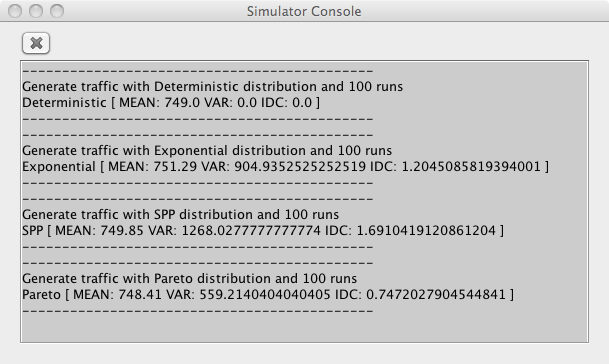
\includegraphics[width=0.9\textwidth]{figures/simconsole.png}
	\end{center}}
	\caption{Confronto dei valori medi di vari tipi di distribuzione}
	\label{fig:random}
\end{figure}
\end{frame}

\section{Simulatore $M/G/1$}
\begin{frame}{Simulatore $M/G/1$}
Sistema a singolo servitore e a singola coda di attesa, con arrivi di tipo poissoniano e tempo di servizio di tipo variabile
\begin{itemize}
	\item Simulazione al variare di $\rho$ in $[0,1]$
	\item Simulazione con tempo di servizio Esponenziale, Deterministico, SPP e di Pareto
\end{itemize}
\begin{figure}[!h]{
	\begin{center}
	   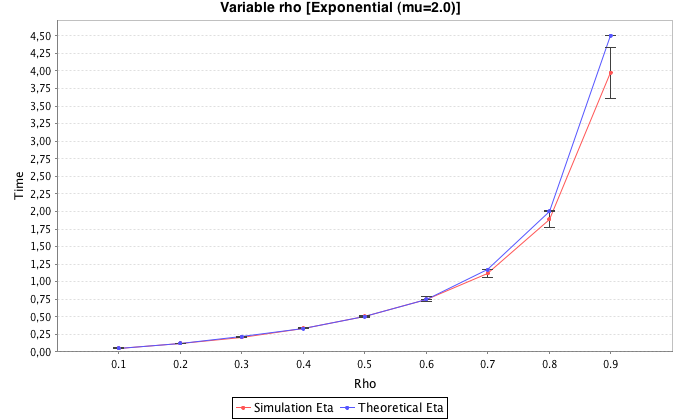
\includegraphics[width=0.45\textwidth]{figures/mg1expmu2.png}
	   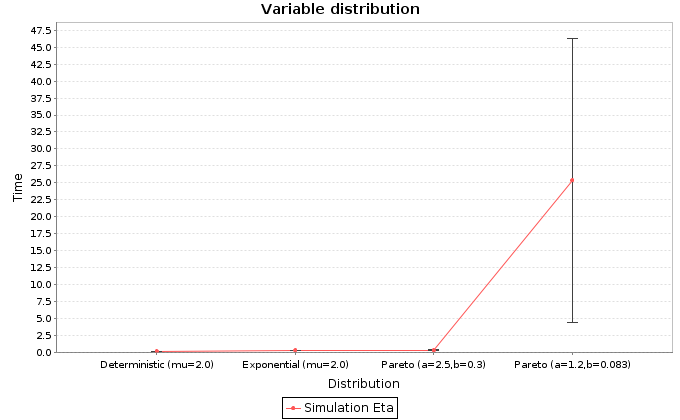
\includegraphics[width=0.45\textwidth]{figures/mg1dists.png}
	\end{center}}
	\caption{Simulazioni $M/G/1$ al variare di $\rho$ e del tipo di distribuzione.}
	\label{fig:random}
\end{figure}
\end{frame}
\begin{frame}{Dettagli tecnici (1/2)}
\vfill
\begin{itemize}
	\item Validazione dei parametri in ingresso, relativamente al tipo di simulazione scelta
	\item Metodi {\tt compareMG1Simulations()} and {\tt simulateMG1WithVariableRho()}
	\item Classe astratta, svincolata dalla particolare politica di gestione delle code, con implementazioni fattorizzate dei metodi comuni
	\item {\tt FCFSSimulator}, implementa anche la possibilit\`a di specificare classi di priorit\`a
\end{itemize}
\vfill
\end{frame}
\begin{frame}{Dettagli tecnici (2/2)}
\vfill
\begin{itemize}
	\item Simulatore di tipo singolo servitore
	\item Singola coda di attesa ordinata in base all'occurrence time
	\item Eventi di tipo arrival and departure, organizzati secondo una gerarchia di classi
	\item Politica di ordinamento specificata in classi wrapper appositamente create, che ereditano da {\tt ComparableEvent}
	\item {\tt OccurrenceTimeComparedEvent}, stabilisce, come politica, un ordinamento semplicemente basato sul tempo di occorrenza dell'evento first-come first-served.
\end{itemize}
\vfill
\end{frame}

% M/G/1 Prio
\section{Simulatore $M/G/1//Prio$}
\subsection{Sistemi $M/G/1/Prio$}
\begin{frame}{Sistemi $M/G/1/Prio$ (1/3)}
Sistemi a singolo servitore con differenti code di attesa, ciascuna delle quali contraddistinta da uno specifico grado di priorit\`a. 
\footnotesize
\begin{table}[!h]
	\begin{center}
	\begin{tabular}{|ccl|}
	\hline
	ID  & n. classi & caratteristiche\\
	\hline
	2 & 2 & $\rho_{1}=x\rho$  \\
	& & $\rho_{2}=(1-x)\rho$ \\
	\hline
	3a & 3 & $\rho_{1}={x\over2}\rho$  \\
	& & $\rho_{2}={x\over2}\rho$  \\
	& & $\rho_{3}=(1-x)\rho$  \\
	\hline
	3b & 3 & $\rho_{1}={x\over10}\rho$ \\
	& & $\rho_{2}={9x\over10}\rho$  \\
	& & $\rho_{3}=(1-x)\rho$  \\
	\hline
	3c & 3 & $\rho_{1}=x\rho$ \\
	& & $\rho_{2}={(1-x)\over2}\rho$  \\
	& & $\rho_{3}={(1-x)\over2}\rho$  \\
	\hline
	\end{tabular}
	\end{center}
	\caption{Caratteristiche delle configurazioni di classi disponibili.}
	\label{tab:mg1prioclasses}
\end{table}
\normalsize
\end{frame}

\begin{frame}{Sistemi $M/G/1/Prio$ (2/3)}
Il parametro $x$ viene fatto variare da $0$ a $1$ con passi di $0.01$
\footnotesize
\begin{figure}[!h]{
	\begin{center}
	   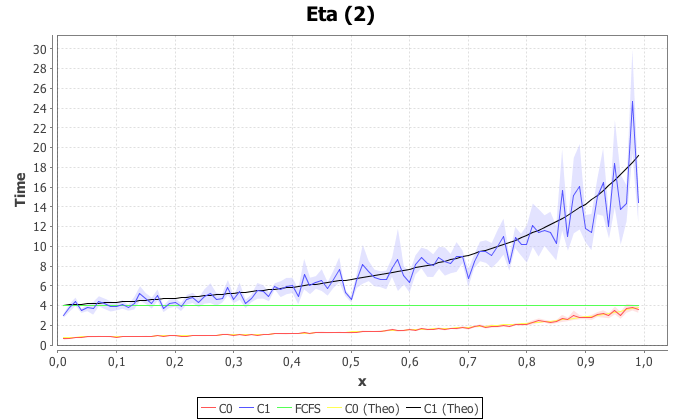
\includegraphics[width=0.85\textwidth]{figures/mg1prio2low.png}
	\end{center}}
	\caption{Tempi medi di attesa nel sistema con coda a due classi}
	\label{fig:mg1prio2low}
\end{figure}
\normalsize
\end{frame}

\begin{frame}{Sistemi $M/G/1/Prio$ (3/3)}
\begin{figure}[!h]{
	\begin{center}
	   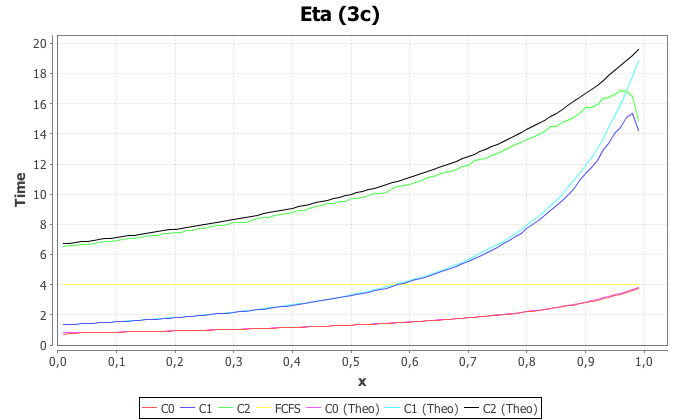
\includegraphics[width=0.9\textwidth]{figures/MG1PRIO3c[mu=2,runs=10000,arrivals=1000].png}
	\end{center}}
	\caption{Tempi medi di attesa nel sistema con coda a tre classi (tipo c)}
	\label{fig:mg1prio3c}
\end{figure}
\end{frame}

\begin{frame}{Precisione}
\vfill
\begin{block}{Nota}
Nel secondo grafico mostrato non si apprezzano a pieno gli intervalli di confidenza. Ci\`o \`e dovuto alla quantit\`a di dati parcolarmente elevata utilizzata, che  ha determinato una notevole precisione dei risultati (oltre ad una notevole durata in termini di tempo di simulazione).
\end{block}
\vfill
\end{frame}

\subsection{Analisi tecnica}
\begin{frame}{Svolgimento della simulazione}
\vfill
Lo svolgimento della simulazione \`e definito all'interno della classe {\tt SimulationRunners} ed \`e suddiviso in due fasi (metodi):
\begin{itemize}
\item {\tt simulateMG1PrioWithVariableRhos(...)}\\
in cui si definiscono le $\rho$ relative alle varie classi.
\item {\tt simulateMG1Prio(...)}\\
in cui si svolge la simulazione vera e propria.
\end{itemize}
\vfill
\end{frame}

% SIMULAZIONI OPZIONALI
\section{Simulazioni opzionali}
\subsection{Stima della probabilit\`a di stato del sistema $M/G/1$}
\begin{frame}{Dettagli tecnici}
\vfill
\begin{itemize}
	\item Valutazione empirica delle probabilit\`a di stato k (numero di utenti presenti nel sistema)
	\item Metodo {\tt simulateMG1EvaluatingProbability()}
	\item Si utilizza {\tt FCFSSimulator} con una sola classe di priorit\`a
	\item Utilizzo del metodo ad-hoc del simulatore, {\tt getStatesProbability}
	\item Tempo totale trascorso nel particolare stato $/$ tempo totale simulazione
\end{itemize}
\vfill
\end{frame}

\begin{frame}{Probabilit\`a di stato}
\begin{figure}[!h]{
	\begin{center}
	   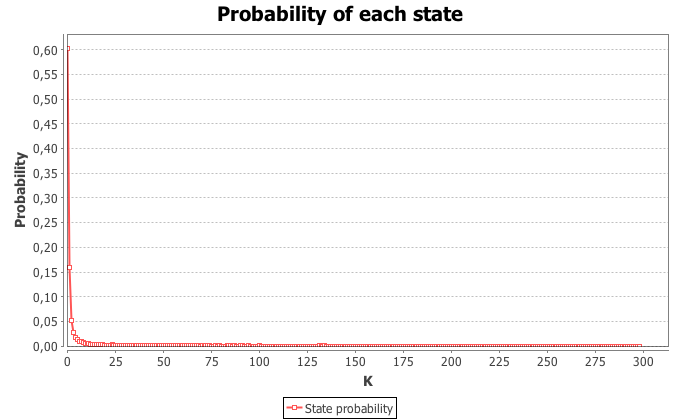
\includegraphics[width=0.5\textwidth]{figures/statepareto.png}
	   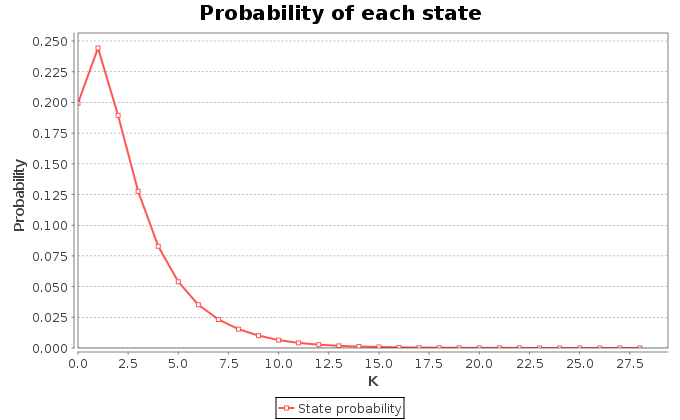
\includegraphics[width=0.5\textwidth]{figures/mg1k.png}
	\end{center}}
	\caption{Probabilit\`a di stato per sistemi con tempi di servizio di Pareto e Deterministici}
	\label{fig:random}
\end{figure}
\end{frame}

\subsection{Sistema $M/G/1$ con politica Shortest Job Next}
\begin{frame}{Simulatore  $M/G/1//SJN$}
\vfill
\begin{itemize}
	\item Sistema a singolo servitore con politica di gestione della coda SJN
	\item Valutazione dell'$\eta$ medio per ogni classe di discretizzazione dei valori di $\theta$
	\item Discretizzazione logaritmica, parametrica
	\item Concentrazione di piccoli intervalli di discretizzazione attorno alla media
	\item Simulazione tramite {\tt SJNSimulator}, che concretizza {\tt Simulator} specializzando la politica di ordinamento della coda mediante la classe ServiceTimeComparedEvent, discendente di ComparableEvent, che ordina in base al tempo di servizio
\end{itemize}
\vfill
\end{frame}

\begin{frame}{$\eta$ medio per SJN}
\begin{figure}[!h]{
	\begin{center}
	   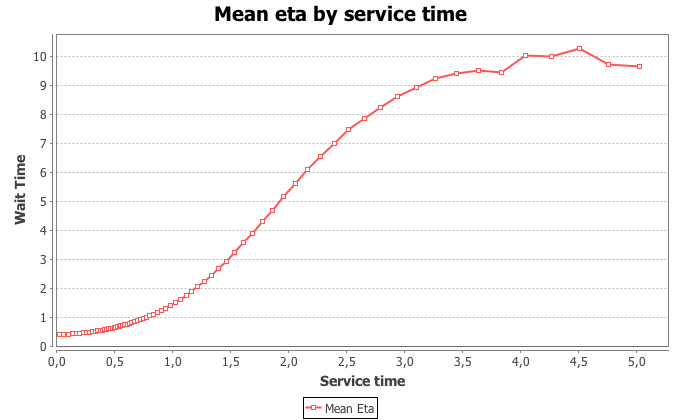
\includegraphics[width=0.9\textwidth]{figures/MG1SJN[rho_08,mu_05,runs_1000,arrivals_100000,steps_30,mult_10].png}
	\end{center}}
	\caption{\footnotesize $\overline{\eta}$ in funzione del tempo di servizio in un sistema con coda SJN}
	\label{fig:random}
\end{figure}
\normalsize
\end{frame}

\begin{frame}{Quantizzatore logaritmico}
\vfill
\begin{itemize}
\item Discretizzazione logaritmica al fine di ottenere una maggiore precisione dei risultati in concomitanza dell'intorno del valor medio di $\theta$
\item Intervalli pi\`u piccoli nei pressi della media, e pi\`u laschi e di dimensioni sempre maggiori allontanandosi da esso
\end{itemize}
\begin{block}{Funzione di discretizzazione}
$f(x) =	\left\{ \begin{array}{rcl}  
	-\log(-x+\overline{\theta}+b) + a + \overline{\theta} & \mbox{for} & x<\theta \\ 
	\log(+x-\overline{\theta}+b) - a + \overline{\theta} & \mbox{for} & x\leq\theta \\ 
	a = \overline{\theta}\cdot \frac{10^{-\overline{\theta}}}{1 - 10^{-\overline{\theta}}} & & \\ 
	b = log(a) \end{array} 
 \right.$ 
\end{block}
\vfill
\end{frame}

% NOTE TECNICHE
\section{Note tecniche generali}
\begin{frame}{Struttura package}
\begin{itemize}
\scriptsize
\item[\textbullet] {\tt gui} \scriptsize{contiene il frame principale del simulatore unitamente alla finestra di console sulla quale vengono visualizzati i messaggi di log}
	\begin{itemize}
	\scriptsize
		\item[\textbullet] {\tt panels} \scriptsize{contiene i differenti pannelli che compongono la finestra principale}
	\end{itemize}
\item[\textbullet] {\tt simulator} \scriptsize{contiene la logica delle differenti simulazioni unitamente al simulatore stesso (con le sue specializzazioni) e classi di supporto per tracciare il progresso delle varie simulazioni}
	\begin{itemize}
	\scriptsize
		\item[\textbullet] {\tt distribution} \scriptsize{contiene la classe astratta {\tt Distribution} e le sue concretizzazioni}
		\item[\textbullet] {\tt events} \scriptsize{contiene gli eventi gestiti dal simulatore unitamente ai wrapper funzionali alla loro politica di ordinamento}
		\item[\textbullet] {\tt misc} \scriptsize{contiene classi di utilit\`a per la realizzazione del simulatore, quali ad esempio il quantizzatore logaritmico e funzionalit\`a statistiche di supporto}
		\item[\textbullet] {\tt random} \scriptsize{contiene le classi utili all'implementazione o incapsulamento dei vari generatori di numeri casuali utilizzati all'interno del simulatore}
	\end{itemize}
\item[\textbullet] {\tt launchers} \scriptsize{contiene gli entry point dell'applicazione, unitamente ad alcune simulazioni notevoli non accedibili mediante interfaccia grafica}
\end{itemize}
\end{frame}

\begin{frame}{Executor}
\vfill
Al fine di scaricare l'onere computazionale derivante dallo svolgimento di ogni singola simulazione esternamente alla \emph{gui} si ricorre all'utilizzo di un \emph{worker-thread} al quale vengono demandati tutti i task esterni all'interfaccia grafica.
\vfill
Particolare tipo di esecutore, {\tt SingleThreadExecutor}, al quale vengono sottomesse tutte le simulazioni
\vfill
Eventuali paramter-checking e feedback visuali vengono lasciati, come di dovere, all'{\tt Event Dispatch Thread}
\vfill
\end{frame}

\begin{frame}{Grafici delle simulazioni}
\vfill
Utilizzo di \emph{JFreeChart \footnote{http://www.jfree.org/jfreechart/}}
	\begin{itemize}
	\footnotesize
		\item[\textbullet] permette la realizzazione di grafici all'interno dell'environment Java
		\item[\textbullet] permette l'esportazione dei grafici prodotti in diversi formati di immagine 
		\item[\textbullet] consente di navigare, ridimensionare, zoomare ed editare i chart tramite interfaccia grafica
	\end{itemize}
\vfill
Vantaggio di poter generare i grafici direttamente da codice, senza bisogno di utilizzare tool esterni e senza dover estrarre ed esportare i dati dal simulatore
\end{frame}

\begin{frame}{Logging delle simulazioni}
\vfill
Utilizzo di una console grafica, di supporto al frame principale, che permette di visualizzare i trace log stampati durante le simulazioni
	\begin{itemize}
		\footnotesize
		\item[\textbullet] aumenta il livello di comprensione delle simulazioni visualizzando i valori precisi sia dei risultati che di alcune fasi intermedie
		\item[\textbullet] bottone ad-hoc nella finestra principale che consente di far apparire/scomparire la console
	\end{itemize}
\vfill
Utilizzo di \emph{log4j \footnote{http://logging.apache.org/log4j/}} per le utility di logging
	\begin{itemize}
	\footnotesize
		\item[\textbullet] permette la realizzazione agile di logging all'interno dell'environment Java
		\item[\textbullet] facilita sia il filtraggio che la specifica della \emph{verbosit\`a} dei log
		\item[\textbullet] permette di redirezionare le entry di log su differenti canali di output in maniera molto agile
	\end{itemize}
\end{frame}

\section{Conclusioni}

\begin{frame}{Conclusioni}
\vfill
Un simulatore di teletraffico aiuta, in generale, l'analisi empirica di sistemi soggetti a traffico i quali, per loro natura, sono relativamente complessi
		\begin{itemize}
		\footnotesize
			\item aiuta a validare modelli che studiano le grandezze di interesse di questi sistemi
			\item permettono di farsi un'idea, in breve tempo, del comportamento del sistema variandone agilmente le condizioni al contorno e di utilizzo
			\item rappresenta una risorsa di indiscutibile utilit\`a per la sintesi ed il dimensionamento di tali sistemi per applicazioni reali, rendedo possibile un'immediata rappresentazione e valutazione di caratteristiche e dinamiche altrimenti difficili da catturare
		\end{itemize}
\vfill
\end{frame}



%dunno what it does... :-O
\section*{}

\section{Bibliografia}
\begin{frame}{Bibliografia}
\begin{itemize}
\item  F. Callegati, G. Corazza
  \emph{``Elementi di teoria del traffico per le reti di telecomunicazioni''}
  Societ\`a Editrice Esculapio, Bologna
  2006

\item
  W. Cerroni
  \emph{- Lucidi del secondo modulo del corso di Progetto di reti di telecomunicazioni -}
  DEIS, Bologna
  2010

\item
  M. Matsumoto, T. Nishimura
  \emph{``Mersenne Twister: A 632-dimensionally equidistribuited uniform pseudorandom number generator''}
  Keio University
  1997

\item
  David Gilbert \emph{``The JFreeChart Class Library - Developer Guide (v.1.0.9)''}
  Object Refinery Limited
  2000-2008
\end{itemize}
\end{frame}


\frame{\titlepage}
\end{document}

%	NOTE

%	\fill
%	\vspace{10}
%	\begin{block}{Introduzione}
%	\begin{itemize}
%		\item 1
%		\item 2
%	\end{itemize}
%	\end{block}

